\icode{N23E-MV-SI-L3-261011-001}
\nceeID[4]{2023湖北}{7}
一列简谐横波沿\(x\)轴正向传播，波长为\qty{100}{cm}，振幅为\qty{8}{cm}。介质中有\(a\)和\(b\)两个质点，其平衡位置分别位于\(x =- \frac{40}{3}\) \,\qty{}{cm}和\(x =\) \,\qty{120}{cm}处。某时刻\(b\)质点的位移为\(y =\) \,\qty{4}{cm}，且向\(y\)轴正方向运动。从该时刻开始计时，\(a\)质点的振动图像为\paren[]
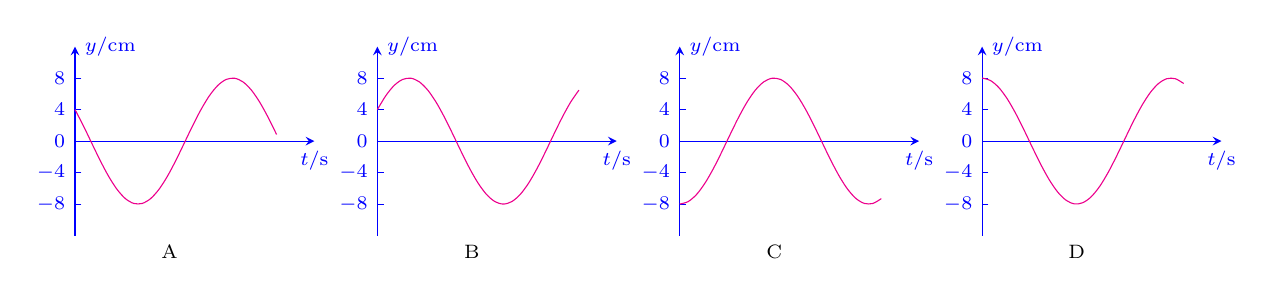
\begin{tikzpicture}[>=stealth,font=\scriptsize]
	\begin{scope}[scale=.8]
		\draw[->,blue] (0,0)--(3.8,0)node[below]{\(t\)/\qty{}{s}};
		\draw[->,blue] (0,-1.5)--(0,1.5)node[right]{\(y\)/\qty{}{cm}};
		\foreach \y/\n in {-1/-8,-.5/-4,0/0,.5/4,1/8}
			\draw[blue] (.1,\y)--(0,\y)node[left]{\(\n\)};
		\draw[domain=0:3.2,smooth,magenta] plot(\x,{cos((2*pi*\x/3+pi/3) r)});
		\node at(1.5,-1.5)[below]{ A};
	\end{scope}
	\begin{scope}[scale=.8,xshift=4.8cm]
		\draw[->,blue] (0,0)--(3.8,0)node[below]{\(t\)/\qty{}{s}};
		\draw[->,blue] (0,-1.5)--(0,1.5)node[right]{\(y\)/\qty{}{cm}};
		\foreach \y/\n in {-1/-8,-.5/-4,0/0,.5/4,1/8}
			\draw[blue] (.1,\y)--(0,\y)node[left]{\(\n\)};
		\draw[domain=0:3.2,smooth,magenta] plot(\x,{sin((2*pi*\x/3+pi/6) r)});
		\node at(1.5,-1.5)[below]{ B};
	\end{scope}
	\begin{scope}[scale=.8,xshift=9.6cm]
		\draw[->,blue] (0,0)--(3.8,0)node[below]{\(t\)/\qty{}{s}};
		\draw[->,blue] (0,-1.5)--(0,1.5)node[right]{\(y\)/\qty{}{cm}};
		\foreach \y/\n in {-1/-8,-.5/-4,0/0,.5/4,1/8}
			\draw[blue] (.1,\y)--(0,\y)node[left]{\(\n\)};
		\draw[domain=0:3.2,smooth,magenta] plot(\x,{-cos((2*pi*\x/3) r)});
		\node at(1.5,-1.5)[below]{ C};
	\end{scope}
	\begin{scope}[scale=.8,xshift=14.4cm]
		\draw[->,blue] (0,0)--(3.8,0)node[below]{\(t\)/\qty{}{s}};
		\draw[->,blue] (0,-1.5)--(0,1.5)node[right]{\(y\)/\qty{}{cm}};
		\foreach \y/\n in {-1/-8,-.5/-4,0/0,.5/4,1/8}
			\draw[blue] (.1,\y)--(0,\y)node[left]{\(\n\)};
		\draw[domain=0:3.2,smooth,magenta] plot(\x,{cos((2*pi*\x/3) r)});
		\node at(1.5,-1.5)[below]{ D};
	\end{scope}
\end{tikzpicture}
\begin{answer}
    A\qquad 提示：\qty{120}{cm}+\(\frac{40}{3}\) \qty{}{cm}\( = \lambda + \frac{1}{3}\lambda\)
\end{answer}